\chapter{Frequency response of the system}

\section{Introduction}

The new governing parameters (\massstiff\ and \massdamp) formulated using the linearised QSS equation in chapter \ref{chap:goven_para} provide a good representation of velocity amplitude and mean power output. In this chapter, the new governing parameters are further analysed by investigating the impact of these parameters with galloping frequency response. 

This chapter is quite brief as it was not the primary objective of this study. However, the investigation into the frequency behaviour was carried out to compliment the understanding of \massstiff\ and \massdamp\ on galloping. 

The flow of this chapter is as follows. An expression for the frequency is formulated based on \massstiff\ and \massdamp\ through the natural time-scales of the system. Data are obtained for frequency by pushing the models to the extreme end in order to find limits where it provides an accurate approximation.This followed by the presentation of results through plots and contour plots in \massstiff\ and \massdamp\ space. Finally the limits of the formulated equation is identified and conclusions are made on the galloping frequency. 


\vspace{15mm}

\section{Formulating the linear frequency of the system}

The process was initiated by considering the linearised galloping equation (Eq:\ref{eqn:eom_linear}). The eigenvalues of the linearised QSS model could be found in equation \ref{eqn:eigs}. The term under the square root (equation \ref{eqn:liner_freq}) of this equation can be used to express the frequency of the system provided that the eigenvalues are complex. 

If this condition (presence of complex eigenvalues)is satisfied, the imaginary component could be identified as the frequency of the system. 

\begin{equation}
\label{eqn:liner_freq}
f = \sqrt{\left[\frac{c-\frac{1}{2}\rho U\mathcal{A}a_1}{(m)}\right]^2-4\frac{k}{(m)}}.
\end{equation}



% % % % % % % % %
By substituting \cstar, \mstar\ and \ustar equation \ref{eqn:liner_freq} could be non-dimensionalised as follows:

\begin{equation}
f = \sqrt{\left[c^*\left(\frac{U}{D}\right) - \frac{1}{2}\frac{a_1}{m^*}\left(\frac{U}{D}\right)\right]^2 - 4\left(\frac{U}{D}\right)^2\frac{2\pi}{U^*}}.
\end{equation}

This can then be rewritten as
\begin{equation}
f = \sqrt{\left(\frac{U}{D}\right)^2\left(c^*-\frac{a_1}{2m^*}\right)^2 - 4\left(\frac{U}{D}\right)^2\left(\frac{2\pi}{U^*}\right)^2}.
\end{equation}
By taking the factor of $U/D$ to the left-hand side
\begin{equation}
\frac{fD}{U} = \sqrt{\left(c^*-\frac{a_1}{2m^*}\right)^2 - 4\left(\frac{2\pi}{U^*}\right)^2}.
\end{equation}
Expanding terms gives
\begin{equation}
\frac{fD}{U} = \sqrt{c^{*2} - \frac{2c^*a_1}{2m^*} + \frac{a_1^2}{4m^{*2}} - \frac{16\pi^2}{U*^2}}.
\end{equation}
Multiplying through by $m*^2$ gives
\begin{equation}
\frac{fD}{U} = \sqrt{c^{*2}m^{*2} - c^*m^*a_1 + \frac{a_1^2}{4} - \frac{16\pi^2m{*^2}}{U^{*2}}}.
\end{equation}


By substituting \massstiff\ and \massdamp\ appropriately the expression of the linear frequency reduced to   
\begin{equation}
\label{eqn:linear_freq_final}
\frac{fD}{U} = \sqrt{\Pi_2^2 - \Pi_2a_1 + \frac{a_1^2}{4} - 4\Pi_1}.
\end{equation}

Thus, from equation \ref{eqn:linear_freq_final} the non-dimensionalised linear frequency of the system could be expressed from the newly formulated terms, \massstiff\ and \massdamp.

\section{Frequency data}

The limiting factor of this equation is the instance where it becomes a real number. Thus, certain questions arise. Does the QSS model predict a frequency beyond this point ?, i.e. after eq:\ref{eqn:linear_freq_final} becomes real. If so, what governs the frequency ? Is this region realistic ? or in other words could this region be identified through DNS simulations. 

\subsection{Comparison of all types of frequencies}

Using different techniques three types of frequencies were found namely \freqlin\ \freqqss\ and \freqdns. For a give value of \massstiff and \massdamp\, the linear frequency \freqlin\ was found by solving equation \ref{eqn:linear_freq_final}. \freqqss was obtained by performing an power spectrum analysis on the output signal of the velocity obtained by numerically solving the quasi-steady sate equation. \freqdns\ was obtained using the similar technique as \freqqss\ but the velocity data was obtained through DNS simulations of fluid-structure interactions. 

	% !TeX spellcheck = en_GB
	\begin{figure}[!htb]
	  \setlength{\unitlength}{\textwidth}
	
	        \begin{picture}(1,0.4)(-0.02,0)
	
	 
	      
	      \put(0.08,0.02){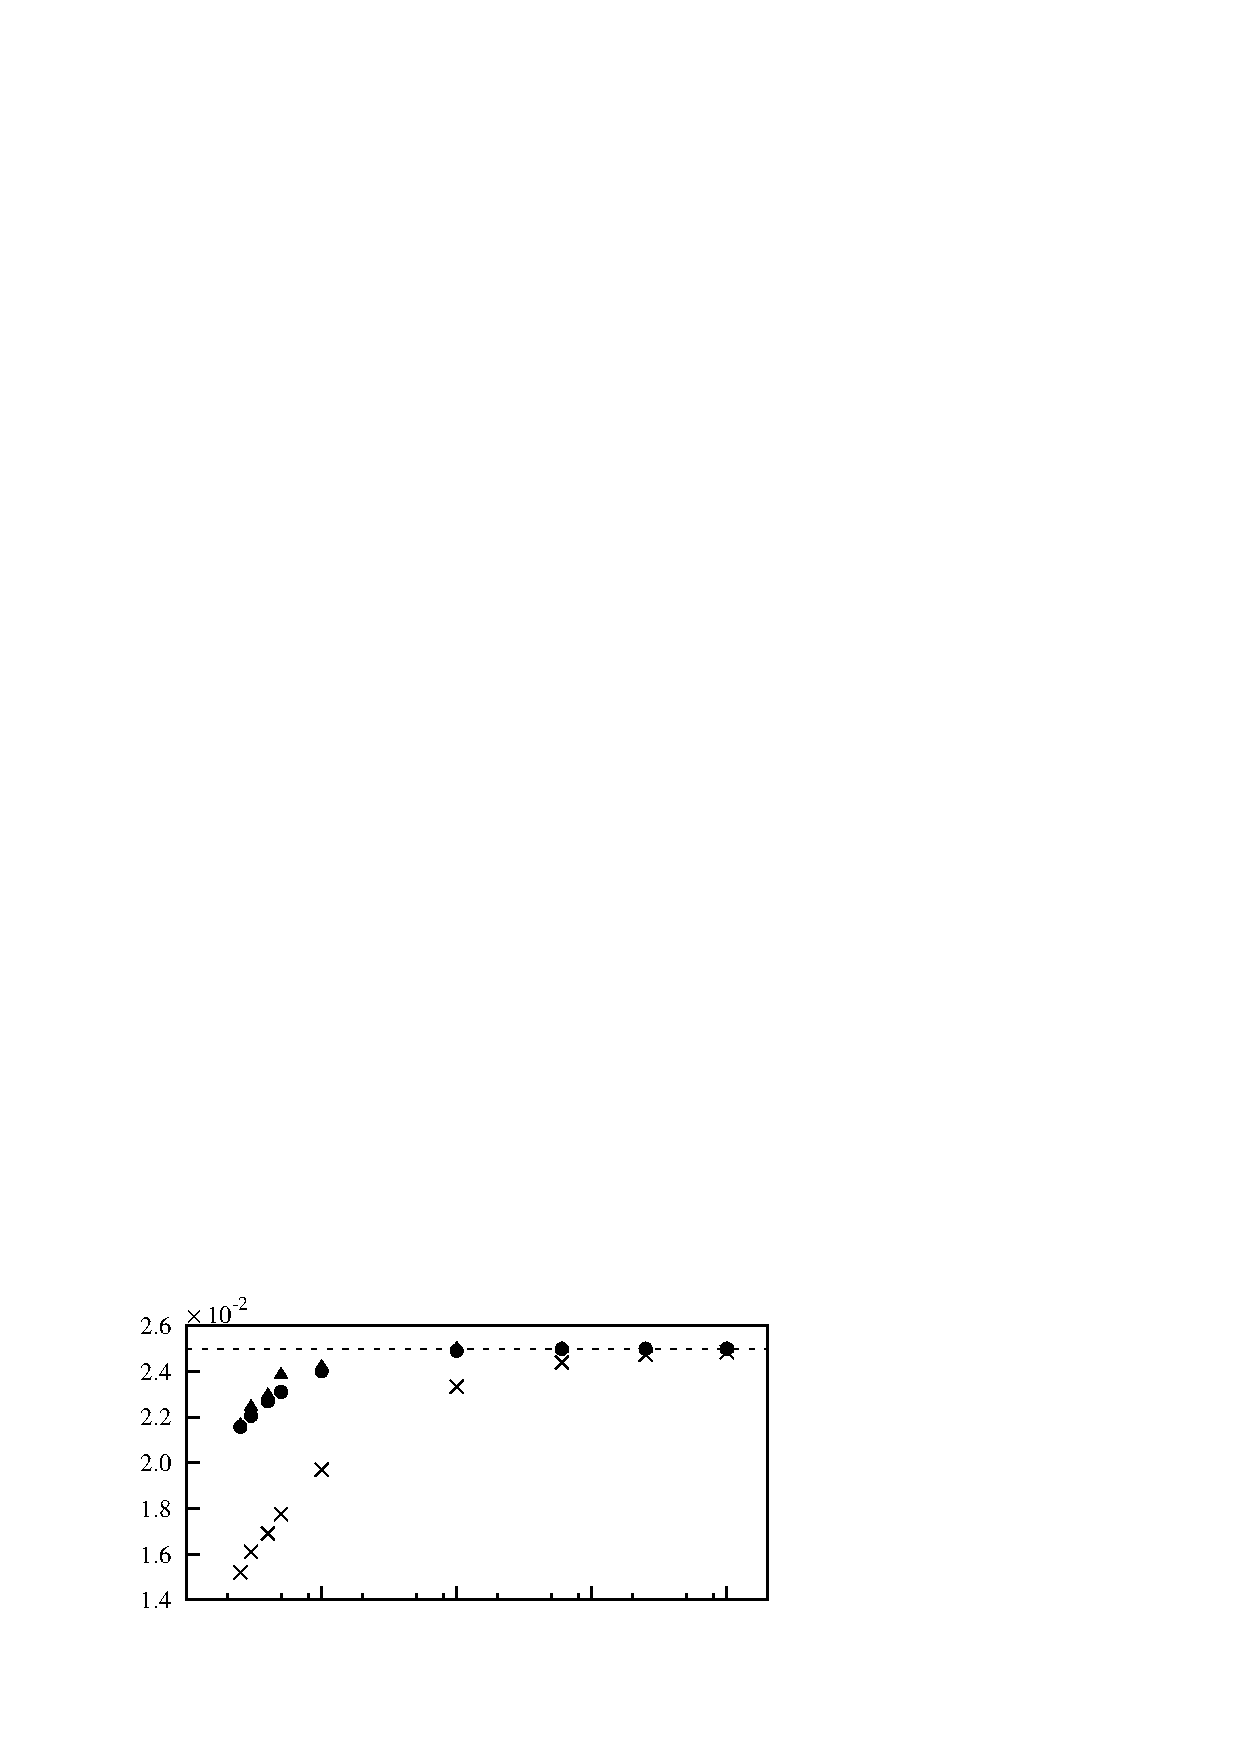
\includegraphics[width=0.75\unitlength]{{./chapter-frequnecy-response/fnp/freq015}.eps}}
	
	      \put(0.47,0.00){\massstiff}
	      
	      
	     
	       \put(0.06,0.235){$\displaystyle\frac{f_{i}}{f}$}
	      
	
	      %\put(0.095,0.218){\small(a)}
	      %\put(0.565,0.218){\small(b)}
	      
	    \end{picture}
	
	  \caption{Frequency ratio as a function of \massstiff. Frequency obtained using QSS simulations, DNS simulations and the linear frequency equation (Eq:\ref{eqn:linear_freq_final})normalised by the undamped natural frequency $f$. $f_{i}$ is the type of frequency i.e. \freqdns,\freqqss ,\freqlin. Data present $\frac{f_{lin}}{f}$ ($\bullet$), $\frac{f_{QSS}}{f}$ (\ding{115}) and $\frac{f_{DNS}}{f}$ ($\times$) at $\massdamp=0.15$, $\reynoldsnumber=200$ and undamped natural frequency, $f=0.025$. }
	    \label{fig:pi2-015-freq}
	\end{figure}
	
	 %vspace{10cm}


The different frequencies normalised by the undamped natural frequency $f$ as a function of \massstiff\ is presented in figure \ref{fig:pi2-015-freq}. It is to be noted that the undamped natural frequency was kept constant at $f=0.025$. The frequency obtained using DNS \freqdns\ is the first to deviate followed by \freqqss\ and then \freqlin. The early deviation of \freqdns could be due to the non linear interaction between the galloping and other forms of forcing such as vortex shedding.

Given the circumstances two regions of frequency response could be identified namely, the linear region where a $f_{lin}>0$ and the non-linear region where $f_{lin}=0$. The data of these two regions are discussed separately.

\subsection{Linear frequency region}

Figure \ref{eqn:liner_freq} shows the frequency ration between \freqlin\ and \freqqss at the region where $f_{lin}>0$. 
	% !TeX spellcheck = en_GB
	\begin{figure}[!htb]
	  \setlength{\unitlength}{\textwidth}
	
	        \begin{picture}(1,0.75)(-0.02,-0.02)
	
	 
	      
	      \put(0.08,0.03){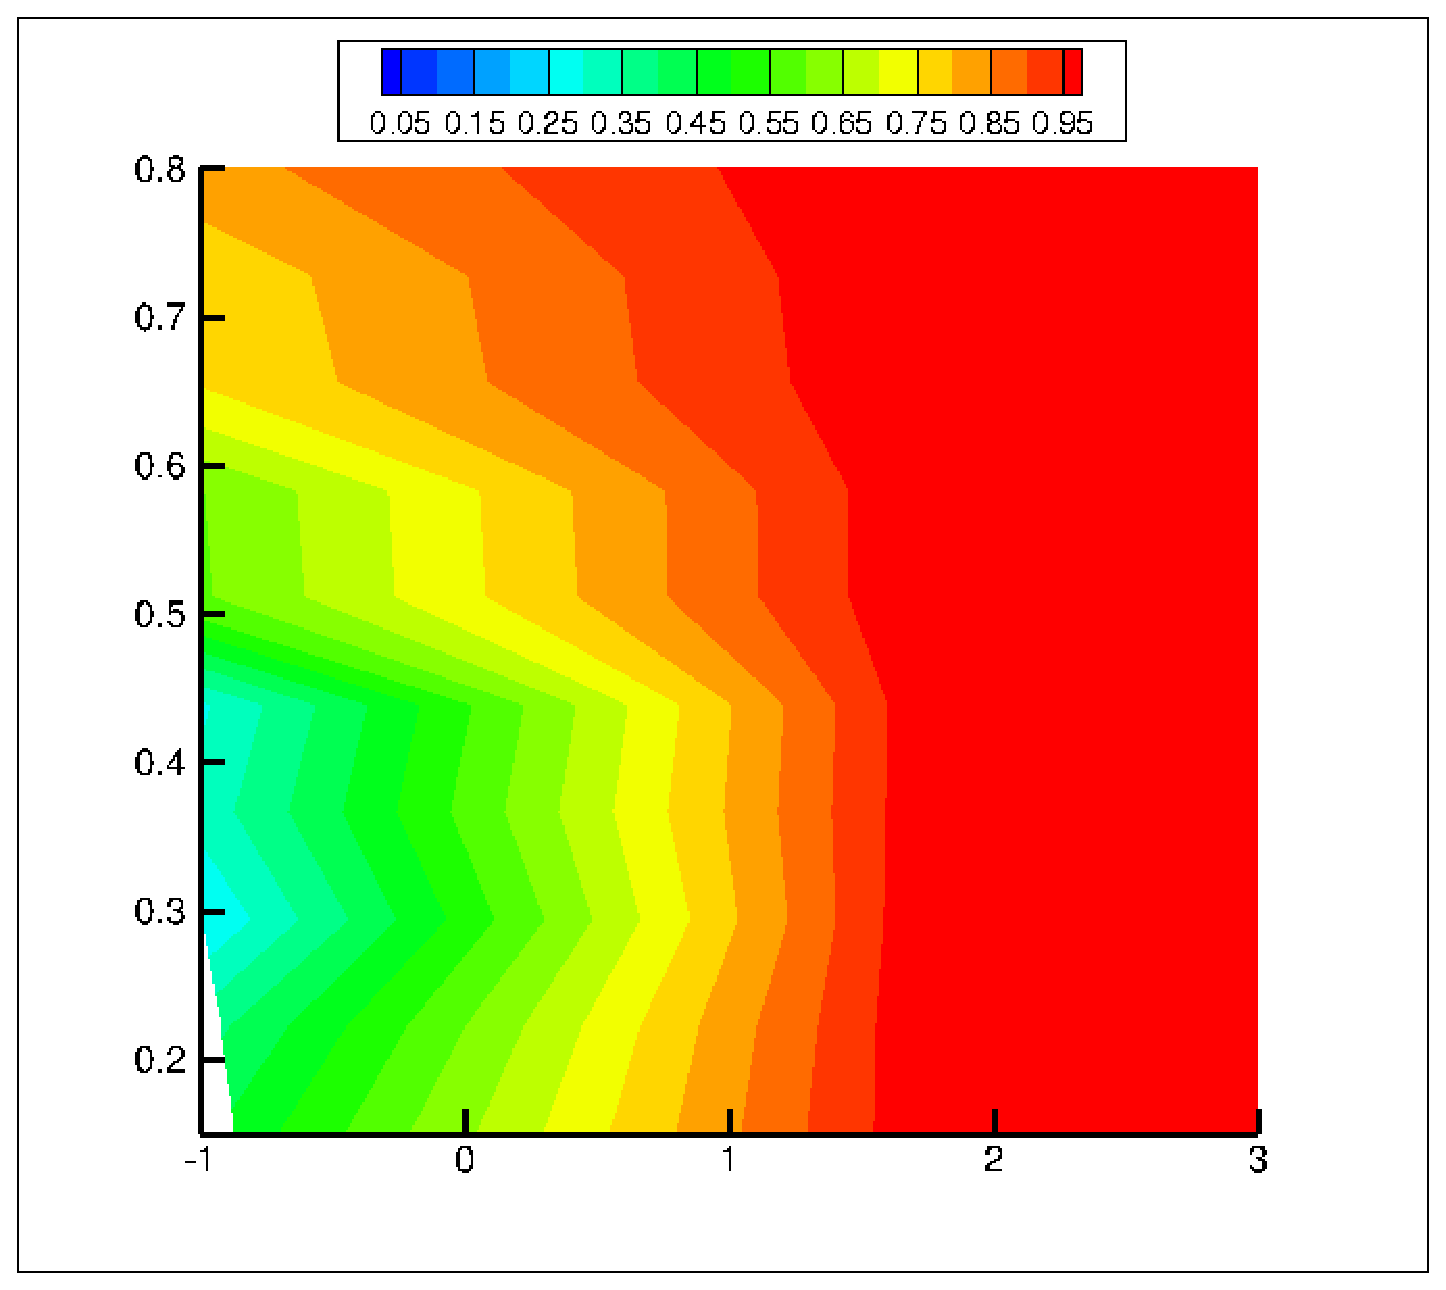
\includegraphics[width=0.75\unitlength]{./chapter-frequnecy-response/fnp/flin-fqss.eps}}
	
	      \put(0.01,0.35){\massdamp}
	      \put(0.46,0.00){$\log(\massstiff)$}
	      \put(0.18,0.65){$\frac{f_{lin}}{f_{QSS}}$}
	      
	      
	     
	       
	      
	
	      %\put(0.095,0.218){\small(a)}
	      %\put(0.565,0.218){\small(b)}
	      
	    \end{picture}
	
	  \caption{Contour plot of  $\frac{f_{lin}}{f_{QSS}}$ in $\log(\massstiff)$\ \massdamp\ space. The linear frequency \freqlin\ provides a good agreement with the frequency predicted by the quasi-steady state model beyond $\massstiff=10$}
	    \label{fig:freq-qss-linear}
	\end{figure}
	
	 %vspace{10cm}


The QSS frequency data tends to agree well between \freqlin\ and \freqqss\ until $\massstiff=10$ for almost all values of \massdamp. As \massstiff\ is further reduced the frequency ratio tends to reduce implying a further deviation between the frequencies.   

	% !TeX spellcheck = en_GB
	\begin{figure}[!htb]
	  \setlength{\unitlength}{\textwidth}
	
	        \begin{picture}(1,0.75)(-0.02,-0.02)
	
	 
	      
	      \put(0.08,0.03){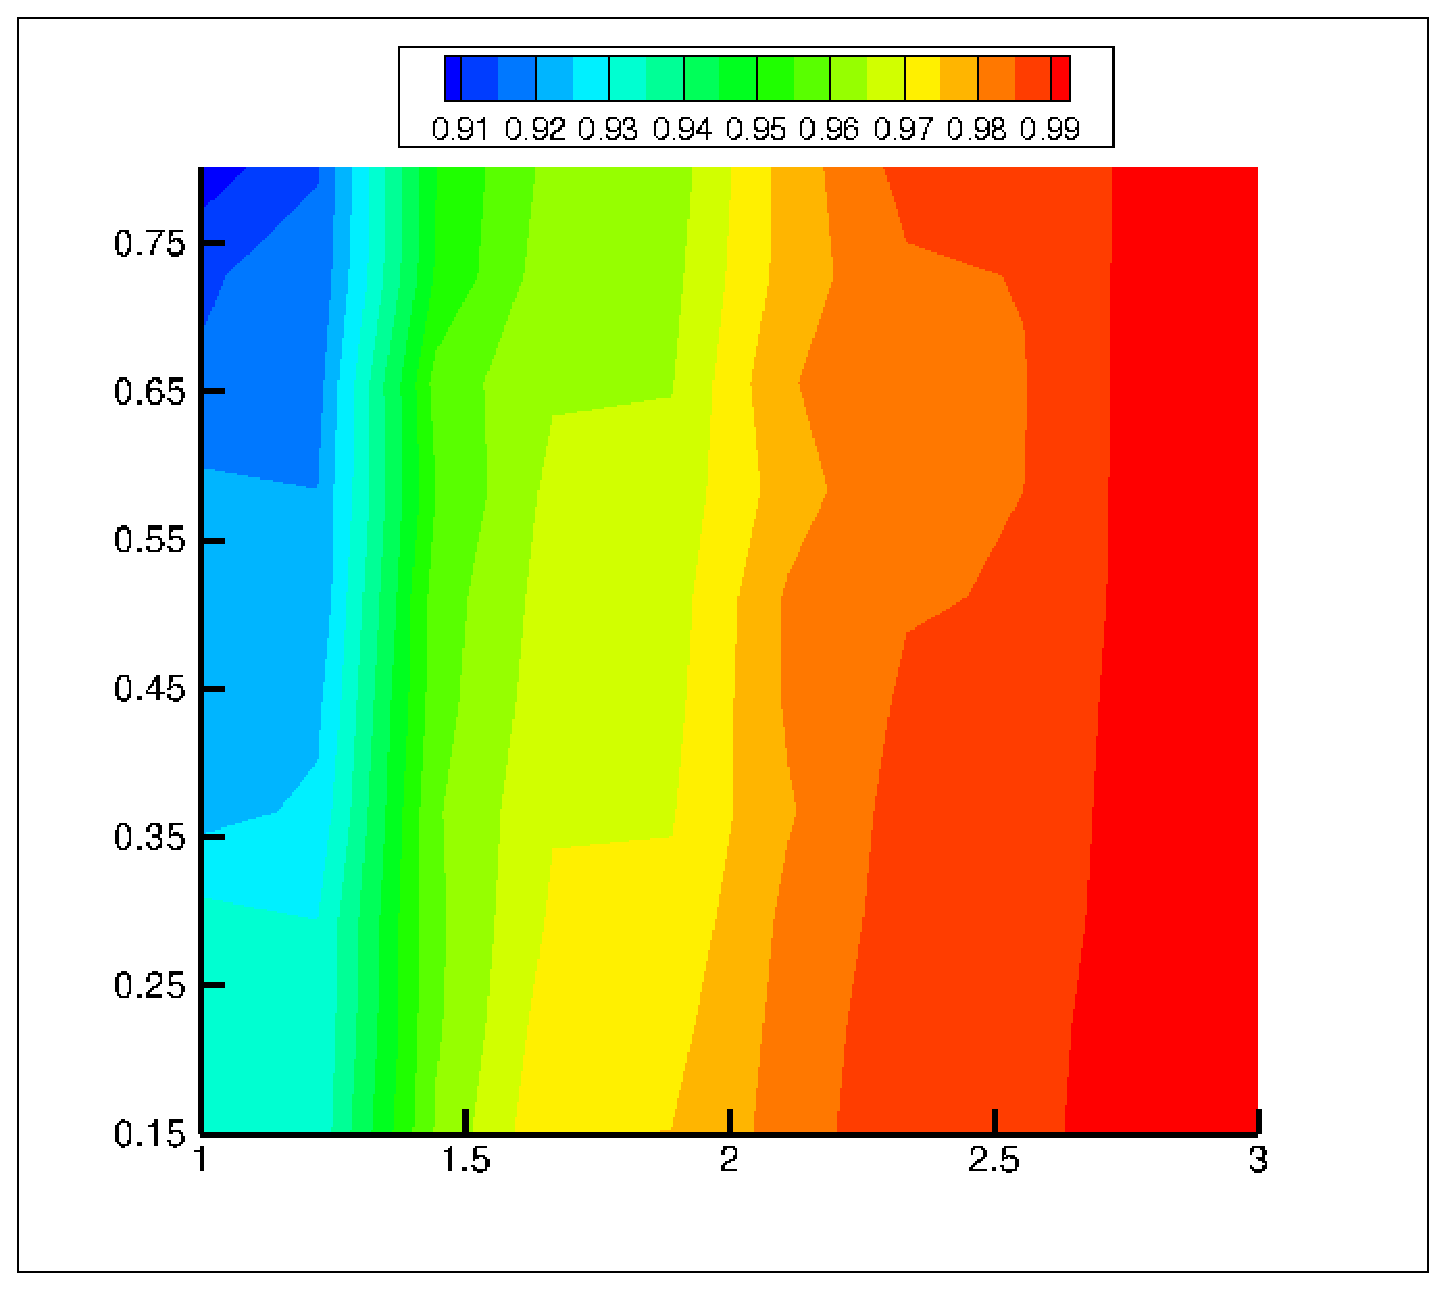
\includegraphics[width=0.75\unitlength]{./chapter-frequnecy-response/fnp/fdns-flinear.eps}}
	
	      \put(0.1,0.36){\massdamp}
	      \put(0.45,0.075){$\massstiff$}
	      \put(0.24,0.67){$\frac{f_{lin}}{f_{DNS}}$}
	      
	     
	       
	      
	
	      %\put(0.095,0.218){\small(a)}
	      %\put(0.565,0.218){\small(b)}
	      
	    \end{picture}
	
	  \caption{Contour plot of  $\frac{f_{lin}}{f_{DNS}}$ in $\massstiff$\ \massdamp\ space. The linear frequency \freqlin\ provides a good prediction of the DNS frequency over the range of \massstiff plotted here.}
	    \label{fig:feq-dns}
	\end{figure}
	
	 %vspace{10cm}

 
 This pattern could also be observed for the DNS data (figure \ref{fig:feq-dns}). The two frequencies \freqlin\ and \freqdns\ tend to have a good agreement in the selected space of \massstiff\ and \massdamp\. It should be specially noted that the lower boundary of \massstiff\ was limited ($\massstiff=10$) because of the fact that galloping was weak in the DNS data hence, no galloping frequency could be obtained with the power spectrum analysis. However, there could be other techniques which was non considered here as mention earlier this analysis was a brief study to compliment the understanding of \massstiff\ and \massdamp. 


\subsection{Non-linear frequency region}

Non-linear frequency region is categorised as the region where no linear frequency is predicted or in other words \freqlin$=0$. Even though there was no linear frequency predicted the QSS model provided a signal for velocity and displacement and therefore providing a frequency. 

	% !TeX spellcheck = en_GB
	\begin{figure}[!htb]
	  \setlength{\unitlength}{\textwidth}
	
	        \begin{picture}(1,0.75)(-0.02,-0.02)
	
	 
	      
	      \put(0.08,0.03){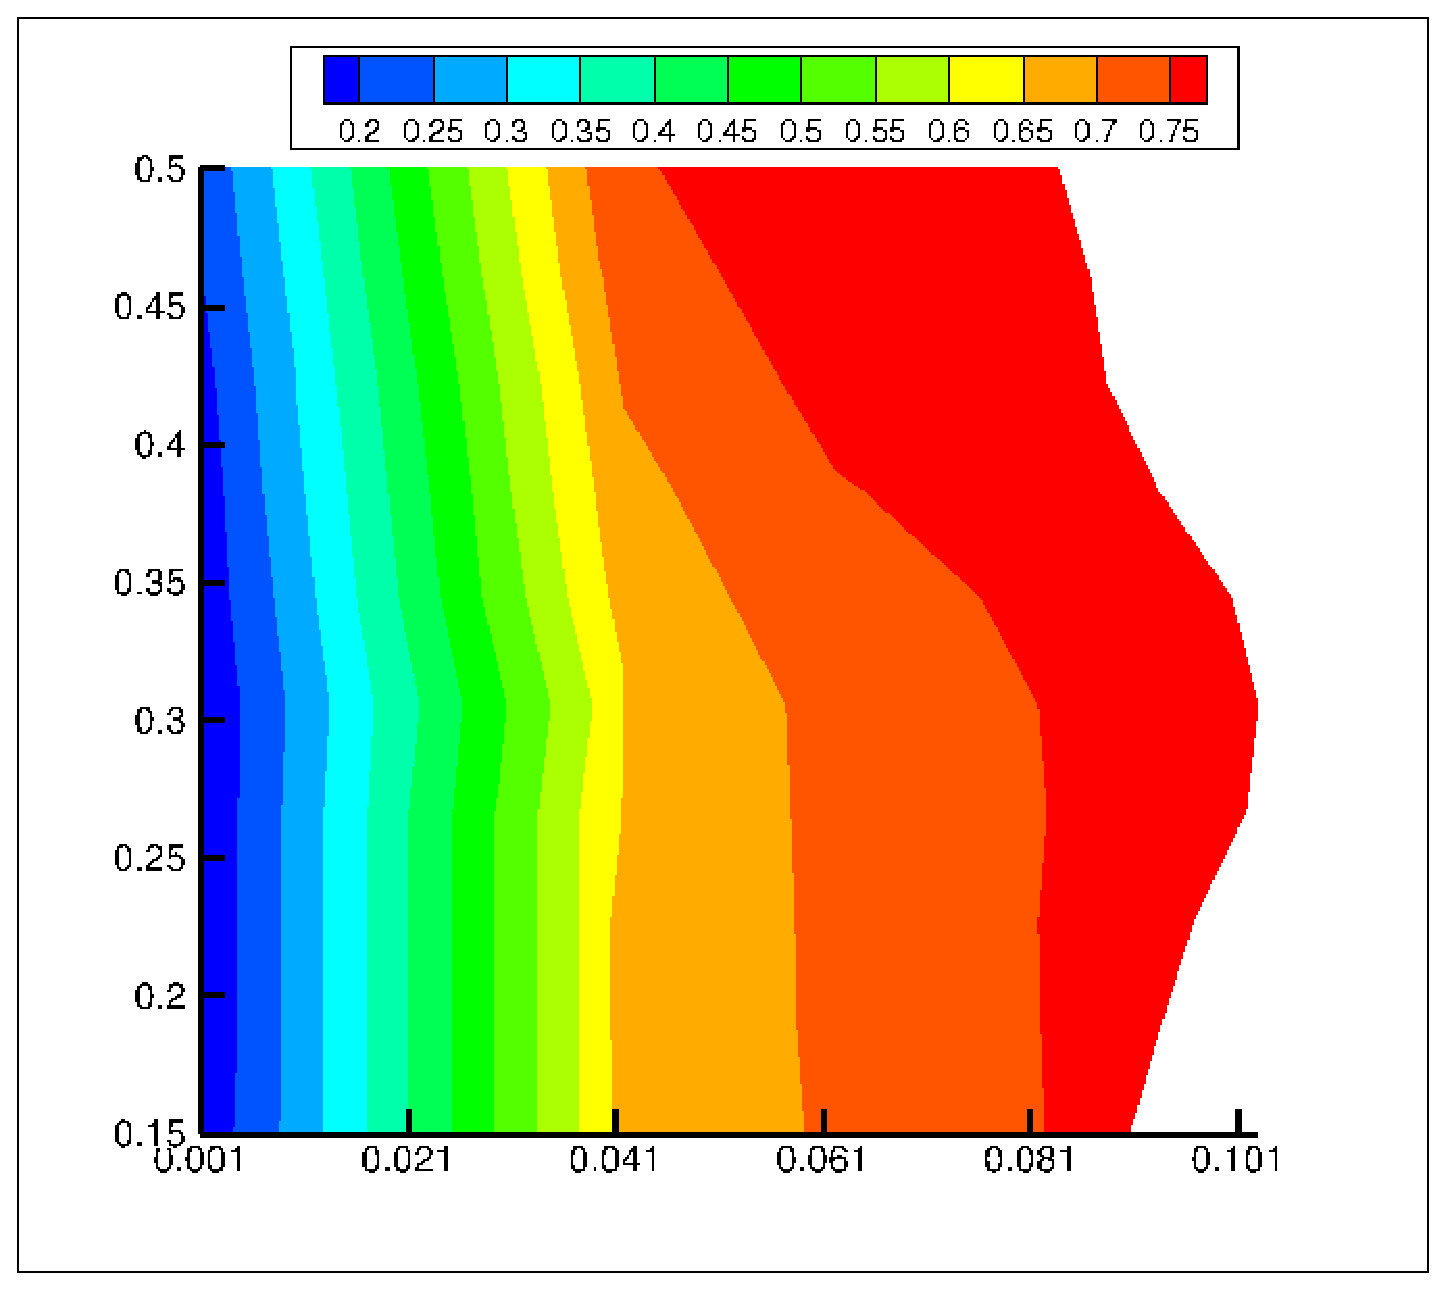
\includegraphics[width=0.75\unitlength]{./chapter-frequnecy-response/fnp/freq_non_linear.eps}}
	
	      \put(0.01,0.35){\massdamp}
	      \put(0.46,0.00){\massstiff}
	      \put(0.17,0.65){$\frac{f_{QSS}}{f}$}
	      
	     
	       
	      
	
	      %\put(0.095,0.218){\small(a)}
	      %\put(0.565,0.218){\small(b)}
	      
	    \end{picture}
	
	  \caption{Contour plot of $\frac{f_{QSS}}{f}$ in \massstiff\ \massdamp\ space, at the region where no linear frequency is predicted ($f_{lin}=0$).}
	    \label{fig:freq_non_linear}
	\end{figure}
	
	 %vspace{10cm}


The frequency ratio $\frac{f_{QSS}}{f}$ tends to deviate as \massstiff\ reduces (Figure \ref{fig:freq_non_linear}) implying more influence of the non-linear terms of the forcing. This region is where the QSS model was pushed to the very extreme end where very large values of \ustar was observed ($\mstar=20$ was kept constant). 

It is to be noted that this non-linear region may not be practical and hence, may not be able to achieve from DNS simulations. Be that as it may, an in-depth analysis should be carried out using some other technique to isolate the weak galloping signal to back this argument. In the current study this was not carried out due fact that it is slightly out of the main scope of the main study and time constrains. 

\section{Summary of the frequency response of the system}

An expression for the frequency of the system was formulated in terms of \massstiff\ and \massdamp\ together with the eigenvalues of the system. The frequency obtained using this expression was termed linear frequency or \freqlin. Two frequency regions were identified namely the linear frequency region and the non-linear frequency region. The linear-frequency region was the region in \massstiff\ and \massdamp\ space where \freqlin$>0$ and the non-linear region was where \freqlin$=0$. The linear frequency agreed well with the DNS results within the boundaries used in the linear frequency region. The lower boundary of \massstiff\ was limited to $\massstiff=10$ as galloping got weaker and vortex shedding got more prominent. The QSS results agreed well for higher values of \massstiff\ in the linear frequency region but tends to deviate as \massstiff\ was reduced. 

QSS frequency was compared with the undamped natural frequency of the system $f$, in the non linear region. This revealed that it had a acceptable agreement with undamped natural frequency of the system in the rage of $0.06\leq\massstiff\leq0.1$ and tends to deviate as \massstiff\ reduced. 

The mere existence of this region was a question as no DNS data could be obtained in this region due to the fact that galloping signal was weak and the techniques used to obtain the  frequency was not sensitive enough to capture these weak signals. Thus it was concluded that further investigations should be carried out on this region but was not pursed in this study due to deviation of the major objective and scope and time constrains.

Be that as it may, The linear expression provided a excellent prediction within the boundaries where DNS data were obtained and therefore complimenting the understanding of the new formulated parameters \massstiff\ and \massdamp.    



